\documentclass[11pt,a4paper]{article}
\usepackage[utf8]{inputenc}
\usepackage[spanish]{babel}	%Idioma
\usepackage{amsmath}
\usepackage{amsfonts}
\usepackage{amssymb}
\usepackage{graphicx} 	%Añadir imágenes
\usepackage{geometry}	%Ajustar márgenes
\usepackage[export]{adjustbox}[2011/08/13]
\usepackage{float}
\restylefloat{table}
\usepackage[hidelinks]{hyperref}
\usepackage{titling}
\graphicspath{{/home/nazaret/Escritorio/LaTEX}}
%\usepackage{minted}
\usepackage{multirow}
\usepackage{caption}
\usepackage{multicol}
\usepackage[shortlabels]{enumitem}
\usepackage{array}
\selectlanguage{spanish}

%Opciones de encabezado y pie de página:
\usepackage{fancyhdr}
\pagestyle{fancy}
\lhead{Nazaret Román Guerrero}
\rhead{Redes Multiservicio}
\lfoot{Grado en Ingeniería Informática}
\cfoot{}
\rfoot{\thepage}
\renewcommand{\headrulewidth}{0.4pt}
\renewcommand{\footrulewidth}{0.4pt}

%Opciones de fuente:
\usepackage[utf8]{inputenc}
\usepackage[default]{sourcesanspro}
\usepackage{sourcecodepro}
\usepackage[T1]{fontenc}

\setlength{\parindent}{15pt}
\setlength{\headheight}{15pt}
\setlength{\voffset}{10mm}

% Custom colors
\usepackage{color}
\definecolor{deepblue}{rgb}{0,0,0.5}
\definecolor{deepred}{rgb}{0.6,0,0}
\definecolor{deepgreen}{rgb}{0,0.5,0}

\usepackage{listings}

\begin{document}
\begin{titlepage}

\begin{minipage}{\textwidth}

\centering

\includegraphics[width=0.5\textwidth]{img/logo.png}\\

\textsc{\Large asignatura\\[0.2cm]}
\textsc{GRADO EN INGENIERÍA INFORMÁTICA}\\[1cm]

{\Huge\bfseries Práctica 2\\}
\noindent\rule[-1ex]{\textwidth}{3pt}\\[3.5ex]
{\large\bfseries Instalación y configuración de un servicio de VoIP mediante servidores SIP}
\end{minipage}

\vspace{1.5cm}
\begin{minipage}{\textwidth}
\centering

\textbf{Autora}\\ {Nazaret Román Guerrero}\\[2.5ex]

\includegraphics[width=0.3\textwidth]{img/etsiit.jpeg}\\[0.1cm]
\vspace{1cm}
\textsc{Escuela Técnica Superior de Ingenierías Informática y de Telecomunicación}\\
\vspace{1cm}
\textsc{Curso 2018-2019}
\end{minipage}
\end{titlepage}

\pagenumbering{gobble}
\pagenumbering{arabic}
\tableofcontents
\thispagestyle{empty}

\newpage

\section{Configuración de usuarios SIP}

Antes de comenzar a configurar usuarios en SIP, reconfiguramos el servicio por si acaso hubiese algo que hubiese sido configurado antes y está mal o no es lo que buscábamos:

\begin{figure}[H]
	\centering
	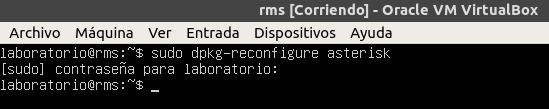
\includegraphics[scale=0.76]{img/1.png}
\end{figure}

Tras hacer esto, comprobamos que el servicio está funcionado correctamente. Lo reiniciamos y probamos a abrir una consola de Asterisk para asegurarnos.

\begin{figure}[H]
	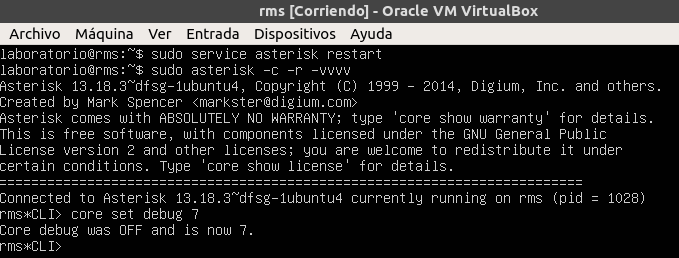
\includegraphics[scale=0.61]{img/2.png}
\end{figure}

Como todo está configurado correctamente, vamos a empezar con los usuarios. Para ello, y siguiendo las instrucciones del propio archivo, creamos una copia del fichero original y creamos uno nuevo y limpio para nuestra configuración.

\begin{figure}[H]
	\centering
	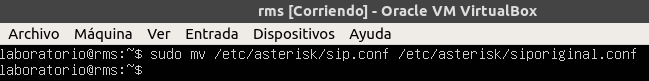
\includegraphics[scale=0.62]{img/3.png}
\end{figure}

Ahora creamos el archivo. En él añadimos contexto general para aquellos usuarios que no tengan un contexto específico. Además vamos a añadir dos usuarios específicos: Pepe y Antonio. Para ello, añadiendo el nombre entre corchetes, indicamos que son usuarios amigos (con \texttt{type}), indicamos sus contraseñas (\texttt{secret}), también indicamos que necesitamos registrar el dispositivo del que llega una llamada (\texttt{host=dynamic}) y finalmente, creamos un contexto para que los dos usuarios puedan contactar entre ellos. El archivo \texttt{sip.conf} queda como sigue:

\begin{figure}[H]
	\centering
	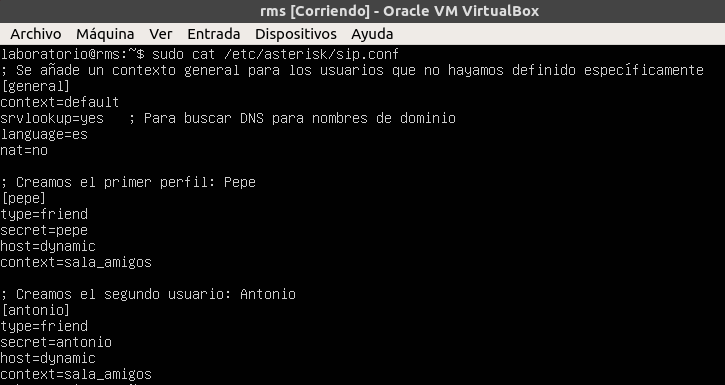
\includegraphics[scale=0.58]{img/4.png}
\end{figure}

Ahora debemos crear un archivo para indicar las acciones que se llevarán a cabo cuando se marque el teléfono de uno de los usuarios. Para ello, hacemos una copia de seguridad del archivo \texttt{/etc/asterisk/extensions.conf} y lo creamos de nuevo limpio.\\

En él indicamos que cada vez que se llame al número 1011 o a ``pepe'' se llame al usuario Pepe. Si se llama al número 1012 o a ``antonio'' se llamará al usuario Antonio.

\begin{figure}[H]
	\centering
	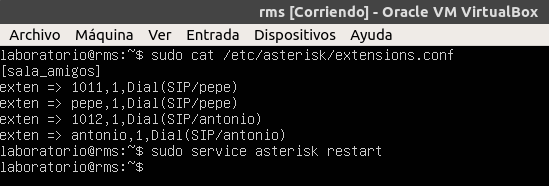
\includegraphics[scale=0.76]{img/6.png}
\end{figure}

Tras esto reiniciamos el servicio y comprobamos si está funcionando correctamente:

\begin{figure}[H]
	\centering
	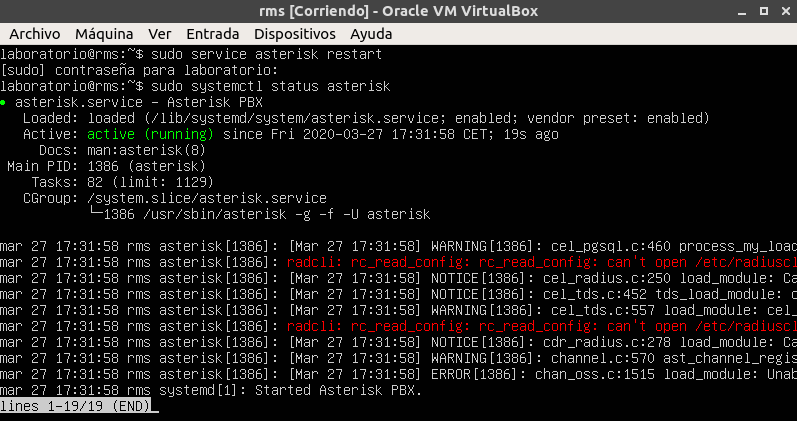
\includegraphics[scale=0.5]{img/5.png}
\end{figure}

Todo está funcionando bien, así que ahora vamos a crear a los usuarios.\\

Primero debemos saber cuál es la IP del servidor con \texttt{ifconfig}, en este caso es \texttt{192.168.56.101}. Ahora creamos los usuarios. Al inicial el cliente, nos pide crear un usuario por primera vez. Lo hacemos igual con los dos usuarios, voy a mostrar el proceso solo con uno de ellos. Introducimos el nombre del usuario.

\begin{figure}[H]
	\centering
	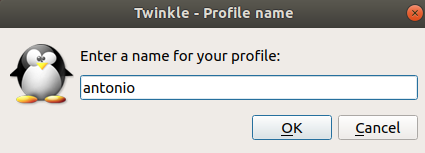
\includegraphics[scale=0.76]{img/9.png}
\end{figure}

Ahora debemos indicar el nombre de usuario definido en el archivo de configuración de SIP, la contraseña e indicar la IP o nombre de domino del servidor. En nuestro caso no tenemos nombre de dominio así que escribimos la IP que hemos sacado antes.

\begin{figure}[H]
	\centering
	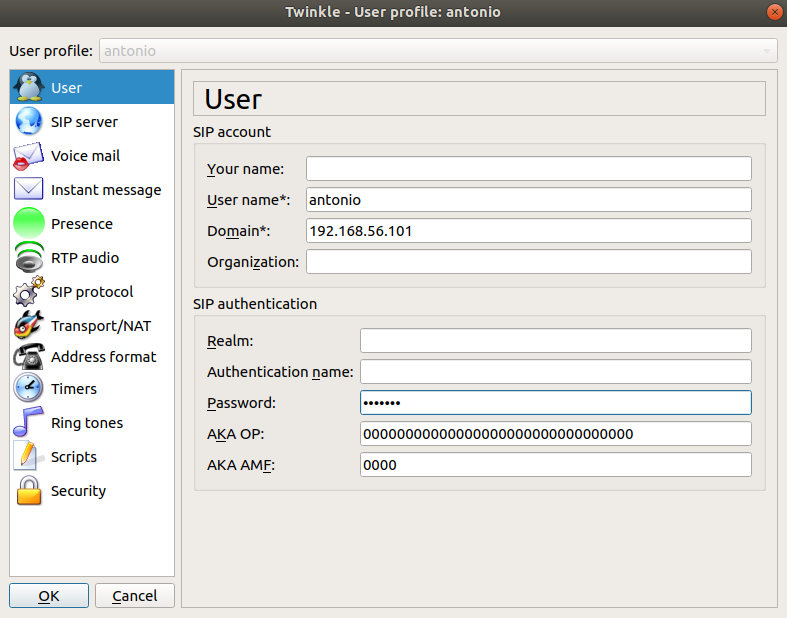
\includegraphics[scale=0.5]{img/10.png}
\end{figure}

Una vez hecho esto, cada vez que iniciemos el dispositivo, se nos pedirá el usuario y la contraseña de nuestro usuario de Twinkle:

\begin{figure}[H]
	\centering
	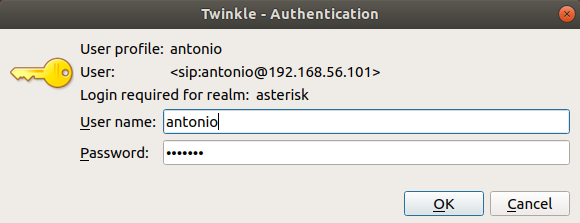
\includegraphics[scale=0.5]{img/12.png}
\end{figure}

Ahora solo queda llamar. Hay un vídeo con una demostración de la llamada en \color{blue}\href{https://drive.google.com/open?id=1scSfceEorV1KhGiVuoRm8_sYQUkKtd5i}{este enlace}. \color{black}

\begin{figure}[H]
	\centering
	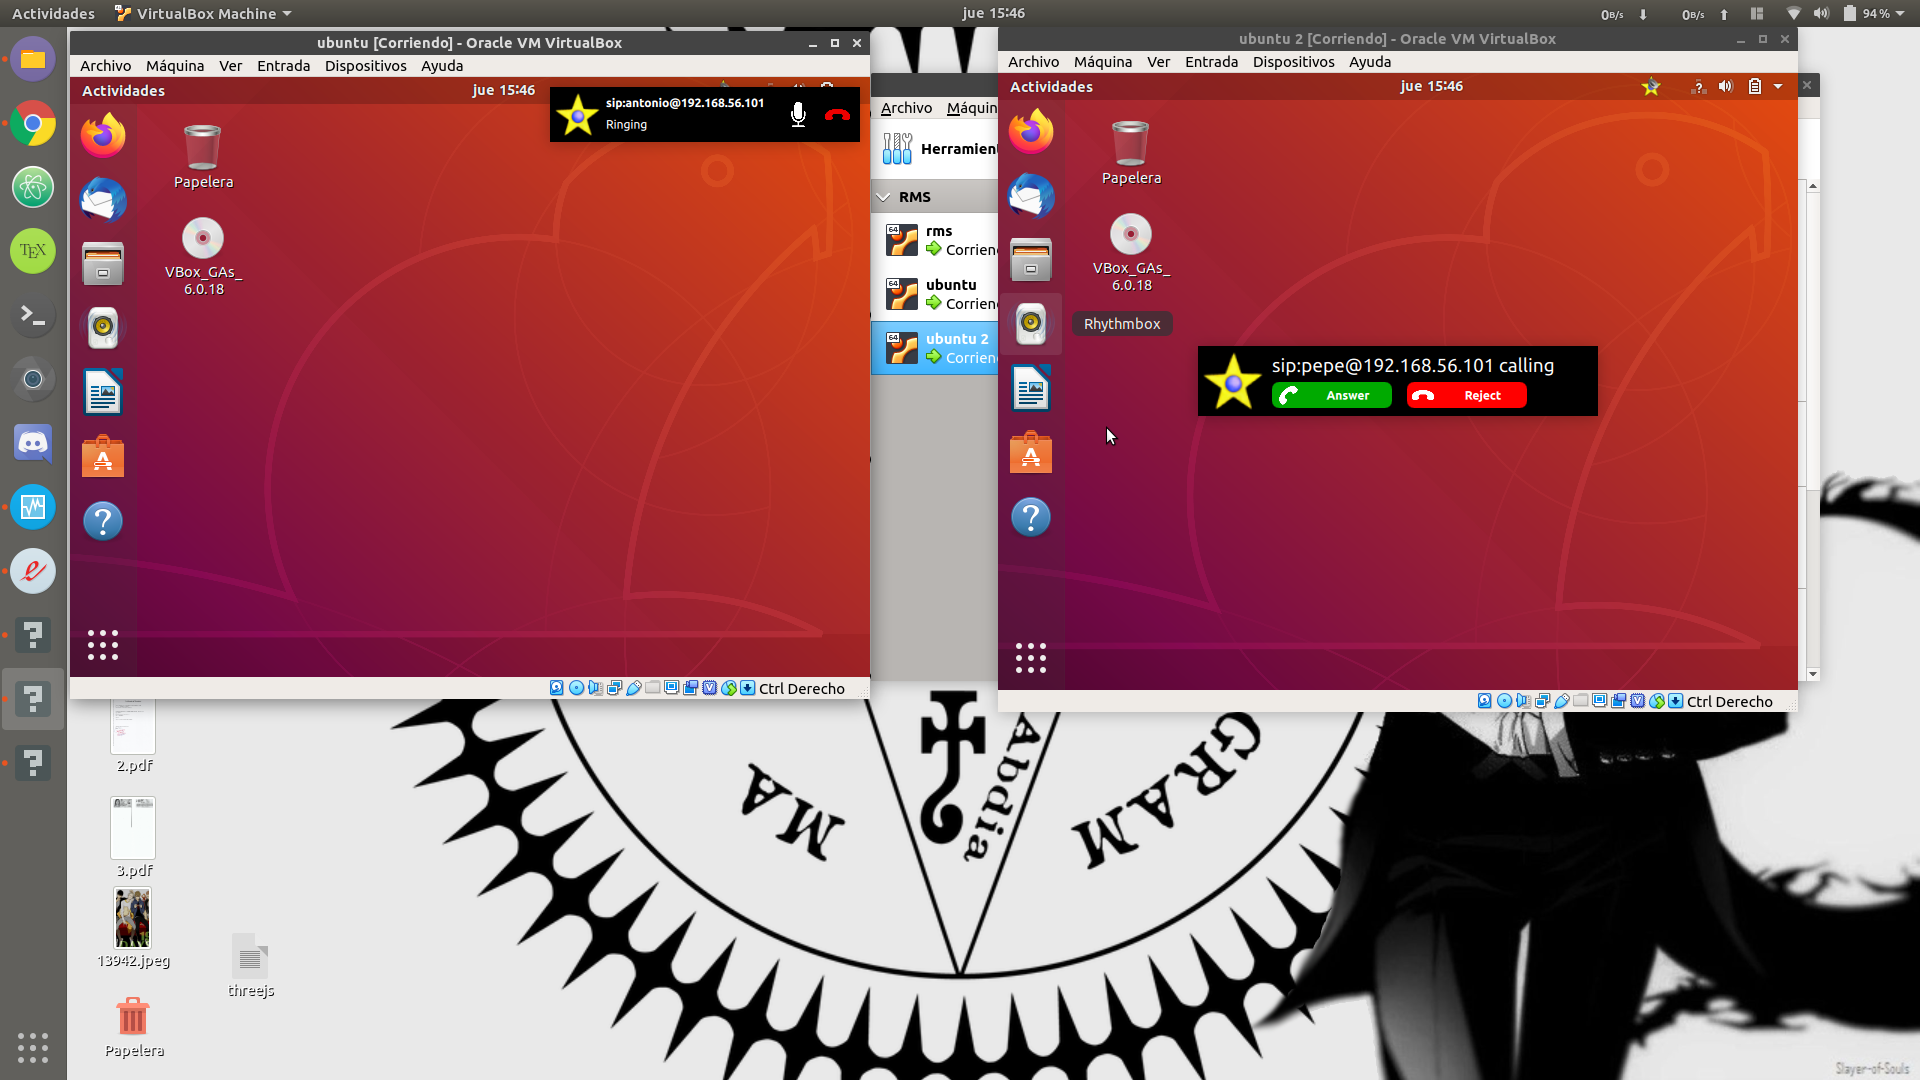
\includegraphics[scale=0.2]{img/13.png}
\end{figure}

Como se puede ver en la imagen y ver y oír en el vídeo, las llamadas entre usuarios funcionan correctamente.

\newpage

\section{Configuración de un menú interactivo}

Ahora vamos a configurar un menú de marcación. Para ello he utilizado Festival, un paquete que viene ya instalado en la máquina servidor que se nos proporciona.\\

Lo primero es hacer un backup del archivo original y crear uno nuevo para configurar Festival y que funcione.

\begin{figure}[H]
	\centering
	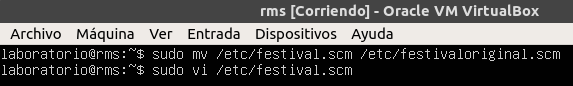
\includegraphics[scale=0.7]{img/14.png}
\end{figure}

Una vez hecho esto, creamos el archivo. En él vamos a indicar cómo va a funcionar Festival. Se definen parámetros como la frecuencia de muestreo, o el servidor donde estará Festival. También se puede definir el lenguaje, dejándolo sin definir por defecto utiliza el inglés. Yo lo he dejado en inglés. Es importante también lanzar el servicio con \texttt{festival --server} (delante de server se escriben dos guiones, aunque en esta memoria parece que solo hay uno).

\begin{figure}[H]
	\centering
	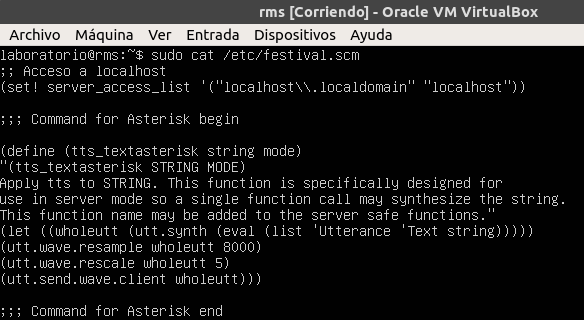
\includegraphics[scale=0.7]{img/15.png}
\end{figure}

Tras hacer esto, debemos añadir nuevas acciones en el archivo \texttt{/etc/asterisk/extensions.conf}. Como la voz no se escucha especialmente bien, es difícil entenderla y es muy gutural (casi me atrevería a decir que parece una psicofonía), he decidido crear un teléfono diabólico. Para llegar a él, debemos marcar el 666 que nos dará indicaciones para marcar distintos números de teléfono en el teclado y que nos digan distintas cosas. He intentado que se escuchara lo mejor posible en los vídeos, pero no he podido mejorarlo, no sé si es problema de mi ordenador o de la configuración de Festival.\\

Lo primero que se hace al llamar al 666 es descolgar la llamada. Se nos dan indicaciones de qué números podemos marcar (aunque se escucha muy mal y casi es difícil entenderlo si no sabes de antemano lo que está diciendo). Se nos dan 30 segundos para marcar un número y tras esto, acaba la llamada.

\begin{figure}[H]
	\centering
	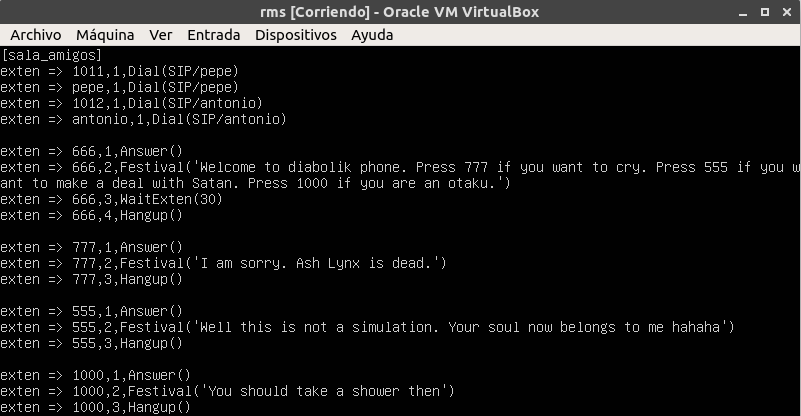
\includegraphics[scale=0.5]{img/16.png}
\end{figure}

Hay una demo con voz en cada una de las marcaciones definidas:

\begin{enumerate}
	\item El 666 nos dirá que si queremos llorar, llamemos al 777, donde nos dirá que el protagonista de una serie ha muerto. Lloré mucho con ese final así que es una buena opción para llorar. Se puede ver \color{blue}\href{https://drive.google.com/open?id=1w3ODj_3aljfEZ5kZcgPZMaOg2Cl3rgpr}{aquí}. \color{black}
	\item Si marcamos el 555 haremos un trato con Satán. Nos dirá que no es una simulación y que ahora nuestra alma le pertenece. Tras esto, se reirá diabólicamente (esta opción es especialmente buena puesto que el hombre al que se escucha hablar da un poco de miedo). Podemos escucharlo \color{blue}\href{https://drive.google.com/open?id=11bMZqrCEVJr9x30LQ493zslP8FdOq8Ds}{aquí}. \color{black}
	\item Finalmente, la opción 1000 nos dirá una frase típica para los fans del anime: que se duchen, porque en las convenciones la verdad es que huele a humano. Esta demo la podemos ver \color{blue}\href{https://drive.google.com/open?id=1uzIh4hmp6K5s--y0RzpPWzXudsFpidG_}{aquí}. \color{black}
\end{enumerate}

\newpage

\section{AGI: Asterisk Gateway Interface}

Finalmente, vamos a hacer una AGI. Para ello, lo primero es saber dónde están situados los archivos de agi, así que tenemos que mirar el archivo de configuración de asterisk, \texttt{/etc/asterisk/asterisk.conf}.

\begin{figure}[H]
	\centering
	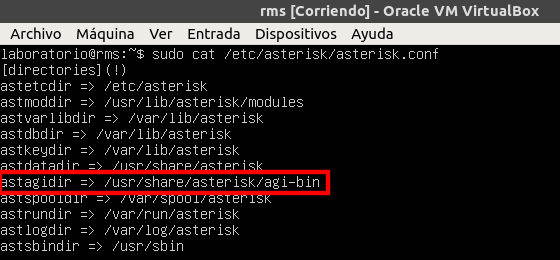
\includegraphics[scale=0.7]{img/17.png}
\end{figure}

Una vez localizado el directorio, creamos una aplicación simple que solo lea una frase que le digamos nosotros y añada un parámetro en dicha frase. Para ello, definimos una variable ``FRASE'' que luego se leerá con Festival. Una vez hecho el programa, lo compilamos y generamos el ejecutable en el directorio donde se guardian los ejecutables de agi.

\begin{figure}[H]
	\centering
	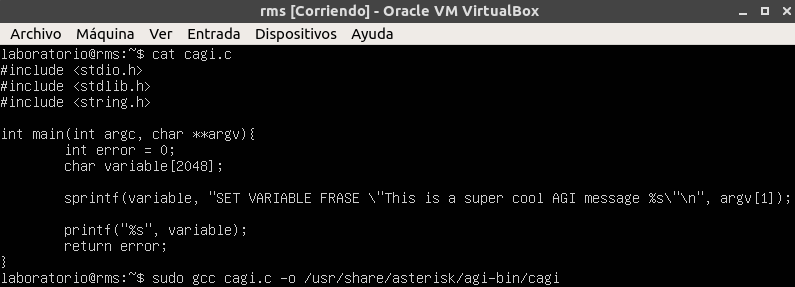
\includegraphics[scale=0.5]{img/18.png}
\end{figure}

Ahora debemos añadir algo más al archivo \texttt{/etc/asterisk/extensions.conf}. Debemos llamar a AGI con el programa y el argumento del programa como parámetros de la llamada. Después con Festival leerémos lo que haya sido escrito por el programa en la salida estándar, en este caso la variable que hemos creado como ``FRASE''. Una prueba del funcionamiento se puede ver \color{blue}\href{https://drive.google.com/open?id=1zSiYJlazfP62NacsPuGumZq_c7zl82Fp}{aquí}. \color{black} El archivo de configuración final es este:

\begin{figure}[H]
	\centering
	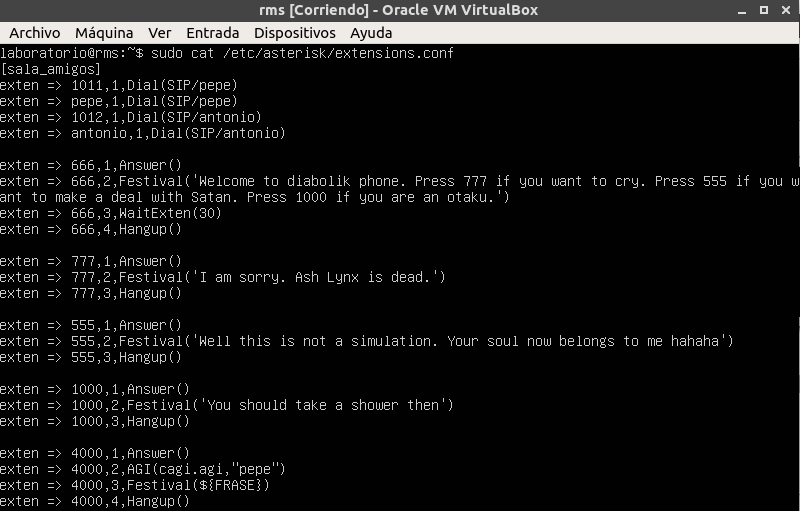
\includegraphics[scale=0.5]{img/19.png}
\end{figure}

\end{document}